\section{Movimiento Armónico}

\subsection{Movimiento Armónico Simple (sin rozamiento)}

Partimos de la segunda ley de Newton con una fuerza recuperadora elástica (Ley de Hooke):
\[
    F = -k u(t), \quad F = m u''(t) \implies m u''(t) + k u(t) = 0
\]

Definiendo la \textbf{pulsación} como $\omega = \sqrt{\frac{k}{m}}$, la ecuación queda:
\[
    u''(t) + \omega^2 u(t) = 0
\]

Para resolverla, proponemos $u(t) = e^{\lambda t}$, lo que nos da el polinomio característico:
\[
    \lambda^2 + \omega^2 = 0 \implies \lambda = \pm i \omega
\]

Usando la fórmula de Euler, la base de soluciones es $\{\cos(\omega t), \sin(\omega t)\}$. La solución general es:
\[
    u(t) = x_1 \cos(\omega t) + x_2 \sin(\omega t), \quad x_1, x_2 \in \mathbb{R}
\]

\textbf{Condiciones iniciales:} Para $u(0) = u_0$ y $u'(0) = v_0$, calculamos:
\begin{itemize}
    \item $u(0) = x_1 \cos(0) + x_2 \sin(0) = x_1 \implies x_1 = u_0$
    \item $u'(t) = -x_1 \omega \sin(\omega t) + x_2 \omega \cos(\omega t) \implies u'(0) = x_2 \omega = v_0 \implies x_2 = \frac{v_0}{\omega}$
\end{itemize}

Por tanto, la solución particular es:
\[
    u(t) = u_0 \cos(\omega t) + \frac{v_0}{\omega} \sin(\omega t)
\]

Para compactar la solución, definimos la \textbf{amplitud} como $A = \sqrt{u_0^2 + (v_0/\omega)^2}$. Si dividimos y multiplicamos por $A$:
\[
    u(t) = A \left[ \frac{u_0}{A} \cos(\omega t) + \frac{v_0/\omega}{A} \sin(\omega t) \right]
\]
Como la suma de los cuadrados de los coeficientes es $\left(\frac{u_0}{A}\right)^2 + \left(\frac{v_0/\omega}{A}\right)^2 = 1$, podemos identificar estos términos con el seno y el coseno de un ángulo $\varphi$ (que se conoce como \textbf{fase inicial}):
\[
    \sin(\varphi) = \frac{u_0}{A}, \quad \cos(\varphi) = \frac{v_0/\omega}{A}
\]
Aplicando la identidad trigonométrica $\sin(\alpha + \beta) = \sin\alpha\cos\beta + \cos\alpha\sin\beta$, llegamos a:
\[
    u(t) = A (\sin(\varphi)\cos(\omega t) + \cos(\varphi)\sin(\omega t)) = A \sin(\omega t + \varphi)
\]

El periodo es $T = \frac{2\pi}{\omega}$, de modo que $u(t + T) = u(t)$:
\[
    u(t + \frac{2\pi}{\omega}) = A \sin(\omega t + 2\pi + \varphi) = A \sin(\omega t + \varphi) = u(t)
\]

\subsection{Conservación de la energía}

Multiplicando la ecuación del movimiento por la velocidad $u'(t)$:
\[
    m u''(t) u'(t) + k u(t) u'(t) = 0
\]
Esto representa la derivada temporal de la energía:
\[
    \frac{d}{dt} \left( \frac{1}{2} m [u'(t)]^2 + \frac{1}{2} k [u(t)]^2 \right) = 0
\]
La energía total ($E_T$) permanece constante:
\[
    E_T = \underbrace{\frac{1}{2} m [u'(t)]^2}_{\text{E. Cinética}} + \underbrace{\frac{1}{2} k [u(t)]^2}_{\text{E. Potencial}} = \frac{1}{2} m v_0^2 + \frac{1}{2} k u_0^2 = \frac{k}{2} \left( \frac{m}{k} v_0^2 + u_0^2 \right) = \frac{k}{2} \left( \frac{v_0^2}{\omega^2} + u_0^2 \right) = \frac{k A^2}{2}
\]

\[
    \frac{m}{2} v^2(t) = \frac{k}{2} (A^2 - u^2(t)) \implies v^2(t) = \frac{k}{m} \left( A^2 - u^2(t) \right) = \omega^2 (A^2 - u^2(t))
\]

\[
    \implies v(t) = \pm \omega \sqrt{A^2 - u^2(t)}
\]

\subsection{Movimiento Armónico Amortiguado}

Partimos de la segunda ley de Newton con una fuerza de rozamiento viscosa proporcional a la velocidad:
\[
    F = -k u(t) - r u'(t), \quad r \text{ es el coeficiente de rozamiento}
\]

\[
    F = m u''(t) \implies m u''(t) + r u'(t) + k u(t) = 0
\]
Como los coeficientes son constantes, proponemos $u(t) = e^{\lambda t}$, lo que nos da el polinomio característico:
\[
    \lambda^2 + \frac{r}{m} \lambda + \frac{k}{m} = 0   
\]
Las raíces de este polinomio característico, $\lambda_1, \lambda_2$ son:
\[
    \lambda_{1,2} = \frac{-\frac{r}{m} \pm \sqrt{\left(\frac{r}{m}\right)^2 - 4 \frac{k}{m}}}{2} = \frac{-r \pm \sqrt{r^2 - 4km}}{2m}
\]
Si $r^2 > 4km$ (resistencia del medio alto), las raíces son reales y negativas, en efecto:

\[
    \lambda_1 = \frac{-r - \sqrt{r^2 - 4km}}{2m} < \frac{-r+\sqrt{r^2 - 4km}}{2m} = \lambda_2 < 0
\]
Solución general: $u(t) = x_1 e^{\lambda_1 t} + x_2 e^{\lambda_2 t}$, con $x_1, x_2 \in \mathbb{R}$. \\
En este caso, el movimiento es \textbf{sobreamortiguado}, y la partícula regresa al equilibrio sin oscilar.

Si $r^2 < 4km$ (resistencia del medio baja), las raíces son complejas conjugadas,
\[
    \lambda_{1,2} = \frac{-r}{2m} \pm i \frac{\sqrt{4km - r^2}}{2m} = -\frac{r}{2m} \pm i \sqrt{\frac{k}{m} - \frac{r^2}{4m^2}}, \qquad \Omega = \sqrt{\frac{k}{m} - \frac{r^2}{4m^2}} = \sqrt{\omega^2 - \frac{r^2}{4m^2}} < \omega
\]

\[
    \lambda_{1,2} = -\frac{r}{2m} \pm i \Omega
\]
Solución general: $u(t) = e^{-\frac{r}{2m} t} (x_1 \cos(\Omega t) + x_2 \sin(\Omega t))$, con $x_1, x_2 \in \mathbb{R}$. \\

\[
    u(t) = e^{-\frac{r}{2m} t} (x_1 \cos(\Omega t) + x_2 \sin(\Omega t)) = e^{-\frac{r}{2m} t} \sqrt{x_1^2 + x_2^2} \left( \frac{x_1}{\sqrt{x_1^2 + x_2^2}} \cos(\Omega t) + \frac{x_2}{\sqrt{x_1^2 + x_2^2}} \sin(\Omega t) \right)
\]

\[
    = e^{-\frac{r}{2m} t} \sqrt{x_1^2 + x_2^2} \sin(\Omega t + \psi) = A e^{-\frac{r}{2m} t} \sin(\Omega t + \psi)
\]

Observemos que la amplitud de la oscilación decrece exponencialmente con el tiempo, debido al factor $e^{-\frac{r}{2m} t}$. 

\[
    \lim_{t \to +\infty} A e^{-\frac{r}{2m} t} \sin(\Omega t + \psi) = 0
\]

En este caso, el movimiento es \textbf{amortiguado}, y la partícula oscila alrededor del equilibrio con una amplitud que decrece exponencialmente.

Este sistema es disipativo, ya que la energía total no se conserva. La energía total en el tiempo $t$ es:
\[
    E_T(t) = \frac{1}{2} m [u'(t)]^2 + \frac{1}{2} k [u(t)]^2
\]
Derivando $E_T(t)$ respecto al tiempo:
\[
    \frac{dE_T}{dt} = m u'(t) u''(t) + k u(t) u'(t) = u'(t) (m u''(t) + k u(t)) = -r [u'(t)]^2 \leq 0
\]
Esto muestra que la energía total del sistema disminuye con el tiempo, lo que es característico de un sistema disipativo.

\subsection{Movimiento Oscilatorio Forzado}

\[
    mu''+ru'+ku = a \sin(\gamma t), \quad a, \gamma \in \mathbb{R} \setminus \{0\}
\]

Sabemos que todas las soluciones de la ecuación homogénea asociada tienen la forma $e^{\lambda t} A \sin(\Omega t + \psi)$.

\[
    u(t) = c_1 \sin(\gamma t) + c_2 \cos(\gamma t) \quad \text{es solución particular de la inhomogénea}
\]

\[
    m(-\gamma^2 c_1 \sin(\gamma t) - \gamma^2 c_2 \cos(\gamma t)) + r(-\gamma c_1 \cos(\gamma t) + \gamma c_2 \sin(\gamma t)) + k(c_1 \sin(\gamma t) + c_2 \cos(\gamma t)) = a \sin(\gamma t)
\]

\[
    \begin{cases}
        (-m \gamma^2 + k) c_1 + r \gamma c_2 = a \\
        (-m \gamma^2 + k) c_2 - r \gamma c_1 = 0
    \end{cases} \qquad \begin{pmatrix}
        -m \gamma^2 + k & r \gamma \\
        -r \gamma & -m \gamma^2 + k
    \end{pmatrix} \begin{pmatrix}
        c_1 \\
        c_2
    \end{pmatrix} = \begin{pmatrix}
        a \\
        0
    \end{pmatrix}
\]

\[
    c_1 = \frac{\begin{vmatrix}
        a & r \gamma \\
        0 & -m \gamma^2 + k
    \end{vmatrix} }{(k - m \gamma^2) + (r \gamma)^2} = \frac{a(k - m \gamma^2)}{(k - m \gamma^2)^2 + (r \gamma)^2}
\]

\[
    c_2 = \frac{\begin{vmatrix}
        -m \gamma^2 + k & a \\
        -r \gamma & 0
    \end{vmatrix} }{(k - m \gamma^2) + (r \gamma)^2} = \frac{a r \gamma}{(k - m \gamma^2)^2 + (r \gamma)^2}
\]

\[
    u(t) = \frac{a(k - m \gamma^2)}{(k - m \gamma^2)^2 + (r \gamma)^2} \sin(\gamma t) + \frac{a r \gamma}{(k - m \gamma^2)^2 + (r \gamma)^2} \cos(\gamma t)
\]

\[
    = \frac{a}{\sqrt{(k - m \gamma^2)^2 + (r \gamma)^2}} \left( \frac{k - m \gamma^2}{\sqrt{(k - m \gamma^2)^2 + (r \gamma)^2}} \sin(\gamma t) + \frac{r \gamma}{\sqrt{(k - m \gamma^2)^2 + (r \gamma)^2}} \cos(\gamma t) \right)
\]

\[
    = \frac{a}{\sqrt{(k - m \gamma^2)^2 + (r \gamma)^2}} \sin(\gamma t + \psi)
\]

Sumamos a la solución homogénea la solución particular que acabamos de encontrar, y obtenemos la solución general:

\[
    u(t) = \underbrace{e^{-\frac{r}{2m} t} \sin(\Omega t + \varphi)}_{\text{régimen transitorio} \xrightarrow{t \uparrow \infty}0} + \underbrace{\frac{a}{\sqrt{(k - m \gamma^2)^2 + (r \gamma)^2}} \sin(\gamma t + \psi)}_{\text{régimen permanente}}
\]

En el estudio de las oscilaciones forzadas, definimos el \textbf{factor de amplificación} como la función $f(\gamma)$, la cual representa la amplitud de la respuesta estacionaria del sistema frente a una excitación externa de frecuencia $\gamma$. Su expresión analítica es:
\[ f(\gamma) = \frac{1}{\sqrt{(k - m \gamma^2)^2 + (r \gamma)^2}} \]
donde $m$ es la masa, $k$ la constante elástica y $r$ el coeficiente de amortiguamiento. A continuación, analizamos el comportamiento de esta función:

\begin{itemize}
    \item \textbf{Simetría y positividad:} La función es par, $f(-\gamma) = f(\gamma) > 0, \forall \gamma \in \mathbb{R}$, lo que indica que la amplitud depende únicamente de la magnitud de la frecuencia.
    \item \textbf{Valores límite:} Cuando la frecuencia externa es nula (fuerza constante), la amplitud es $f(0) = 1/k$ (deflexión estática). Para frecuencias extremadamente altas, la inercia domina y la amplitud tiende a cero: $\lim_{\gamma \to +\infty} f(\gamma) = 0$.
\end{itemize}

\begin{center}
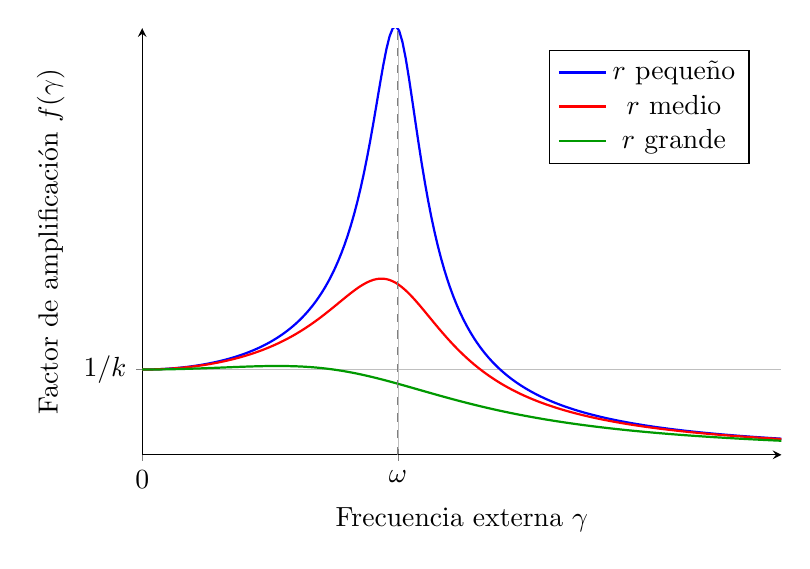
\begin{tikzpicture}
\begin{axis}[
    width=0.8\textwidth, 
    height=7cm,
    samples=200,
    domain=0:2.5,
    ymin=0, ymax=5, % Sustituimos 'restrict y to max' por esto para evitar conflictos
    xlabel={Frecuencia externa $\gamma$},
    ylabel={Factor de amplificación $f(\gamma)$},
    axis lines=left,
    grid=both,
    grid style={line width=.1pt, draw=gray!10},
    major grid style={line width=.2pt, draw=gray!50},
    xtick={0, 1},
    xticklabels={0, $\omega$},
    ytick={1},
    yticklabels={$1/k$},
    legend style={at={(0.95,0.95)}, anchor=north east},
    clip=true
]

% Curva con poco amortiguamiento (Resonancia marcada)
\addplot[thick, blue] {1/sqrt((1 - x^2)^2 + (0.2*x)^2)};
\addlegendentry{$r$ pequeño}

% Curva con amortiguamiento medio
\addplot[thick, red] {1/sqrt((1 - x^2)^2 + (0.5*x)^2)};
\addlegendentry{$r$ medio}

% Curva con mucho amortiguamiento
\addplot[thick, green!60!black] {1/sqrt((1 - x^2)^2 + (1.2*x)^2)};
\addlegendentry{$r$ grande}

% Indicador de la frecuencia natural omega
\draw[dashed, gray] (axis cs:1,0) -- (axis cs:1,5);

\end{axis}
\end{tikzpicture}
\end{center}

Para hallar el valor máximo de la amplitud, buscamos los puntos críticos de $f(\gamma)$. Expresando la función como $f(\gamma) = [(k-m\gamma^2)^2 + (r \gamma)^2]^{-1/2}$, calculamos su derivada respecto a $\gamma$ e igualamos a cero:
\[ f'(\gamma) = -\frac{1}{2} [(k-m\gamma^2)^2 + (r \gamma)^2]^{-3/2} \cdot \left( 2(k-m\gamma^2)(-2m\gamma) + 2 r^2 \gamma \right) = 0 \]
Para que la derivada sea nula, el término entre paréntesis debe ser cero (considerando $\gamma \neq 0$):
\[ -4m\gamma(k - m \gamma^2) + 2 r^2 \gamma = 0 \implies -2m(k - m \gamma^2) + r^2 = 0 \]
Despejando $\gamma^2$, obtenemos la frecuencia de resonancia, que denotaremos como $\gamma_m$:
\[ 2m^2 \gamma^2 = 2mk - r^2 \implies \gamma_m^2 = \frac{k}{m} - \frac{r^2}{2m^2} \]
Utilizando la frecuencia natural del sistema $\omega = \sqrt{k/m}$, la frecuencia donde ocurre el máximo se expresa como:
\[ \gamma_m = \sqrt{\omega^2 - \frac{r^2}{2m^2}} \]
Es importante notar que para que exista un máximo real (pico de resonancia), debe cumplirse que $\omega^2 > \frac{r^2}{2m^2}$. Se observa que $\gamma_m < \Omega < \omega$, donde $\Omega = \sqrt{\omega^2 - \frac{r^2}{4m^2}}$ es la frecuencia natural amortiguada.

Sustituyendo $\gamma_m$ en la función original para hallar el valor máximo del factor de amplificación:
\[ f(\gamma_m) = \frac{1}{\sqrt{(k - m \gamma_m^2)^2 + (r \gamma_m)^2}} = \frac{1}{\sqrt{\left(\frac{r^2}{2m}\right)^2 + r^2 \left(\omega^2 - \frac{r^2}{2m^2}\right)}} \]
Simplificando el radicando:
\[ f(\gamma_m) = \frac{1}{\sqrt{\frac{r^4}{4m^2} + r^2 \omega^2 - \frac{r^4}{2m^2}}} = \frac{1}{\sqrt{r^2 \omega^2 - \frac{r^4}{4m^2}}} = \frac{1}{r \sqrt{\omega^2 - \frac{r^2}{4m^2}}} \]
Dado que el término bajo la raíz es precisamente $\Omega$, concluimos que:
\[ f(\gamma_m) = \frac{1}{r \Omega} \]
Este valor representa el pico máximo de la oscilación. En el límite donde el amortiguamiento desaparece ($r \to 0$), se observa que $\Omega \to \omega$ y $f(\gamma_m) \to +\infty$. Este fenómeno se denomina \textbf{resonancia pura}, donde la sincronización entre la fuerza externa y la frecuencia natural provoca una transferencia de energía teóricamente infinita al sistema.
